
%(BEGIN_QUESTION)
% Copyright 2014, Tony R. Kuphaldt, released under the Creative Commons Attribution License (v 1.0)
% This means you may do almost anything with this work of mine, so long as you give me proper credit

Skisser fasordiagrammer for både fasespenning og fasestrøm i dette balanserte trefasesystemet:

$$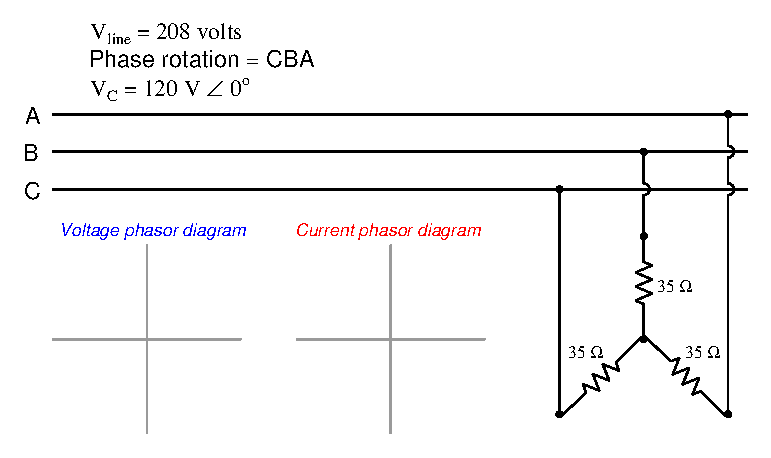
\includegraphics[width=15.5cm]{i00833x01.eps}$$

\vskip 10pt

Anta nå at lasten fjernes fra systemet og at en lavohmig feil oppstår mellom fase B og C. Skisser fasordiagrammer for både fasespenning og fasestrøm, forutsatt at kildegeneratoren er ``stiv'' (dvs. spenningen synker ikke merkbart selv ved stor belastning):

$$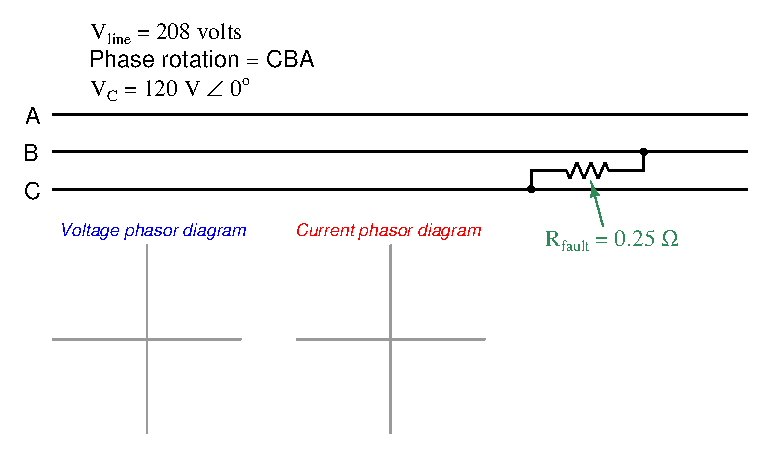
\includegraphics[width=15.5cm]{i00833x03.eps}$$

\underbar{file i00833}
%(END_QUESTION)





%(BEGIN_ANSWER)

Siden motstander ikke gir faseskift mellom spenning og strøm, beholder hver fasestrøm samme fasevinkel som tilsvarende fasespenning:

$$I_A = {V_A \over R_A} = {120 \hbox{ V} \angle 120^o \over 35 \> \Omega \angle 0^o} = 3.43 \hbox{ A} \angle 120^o$$

$$I_B = {V_B \over R_B} = {120 \hbox{ V} \angle -120^o \over 35 \> \Omega \angle 0^o} = 3.43 \hbox{ A} \angle -120^o$$

$$I_C = {V_C \over R_C} = {120 \hbox{ V} \angle 0^o \over 35 \> \Omega \angle 0^o} = 3.43 \hbox{ A} \angle 0^o$$

$$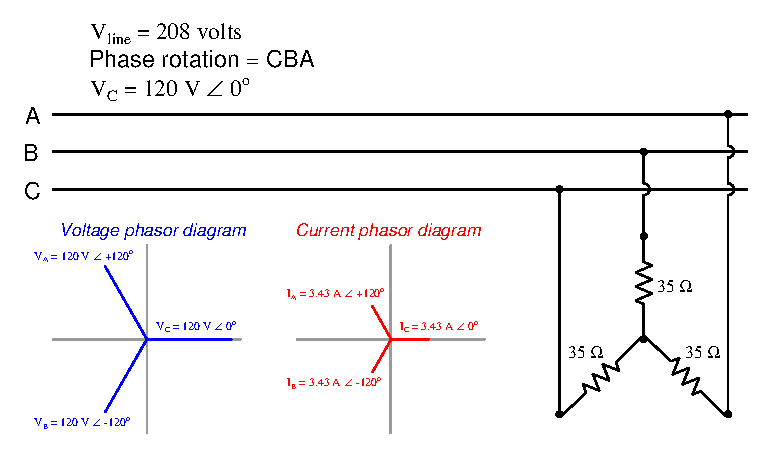
\includegraphics[width=15.5cm]{i00833x02.eps}$$

\vskip 10pt

\filbreak

Situasjonen ved en resistiv fase-til-fase-feil er annerledes. Motstanden ser full linjespenning (208 V), ikke fasespenning (120 V). I tillegg er fasevinkelen en annen: fordi fasoren går mellom endepunktene til B- og C-fasorene, får $V_{BC}$ (rød ledning på B, svart på C) fasevinkel $-150^o$.

Fasestrømmen i leder B beregnes ved å dele $V_{BC}$ på feilresistansen 0.25 $\Omega$:

$$I_B = {V_{BC} \over R_{fault}} = {208 \hbox{ V} \angle -150^o \over 0.25 \> \Omega \angle 0^o} = 832 \hbox{ A} \angle -150^o$$

Fasestrøm i leder C må beregnes fra den fasens perspektiv. $V_{CB}$ peker motsatt vei av $V_{BC}$ og har derfor vinkel +30$^{o}$, ikke $-150^o$. Igjen med Ohms lov:

$$I_C = {V_{CB} \over R_{fault}} = {208 \hbox{ V} \angle 30^o \over 0.25 \> \Omega \angle 0^o} = 832 \hbox{ A} \angle 30^o$$

$$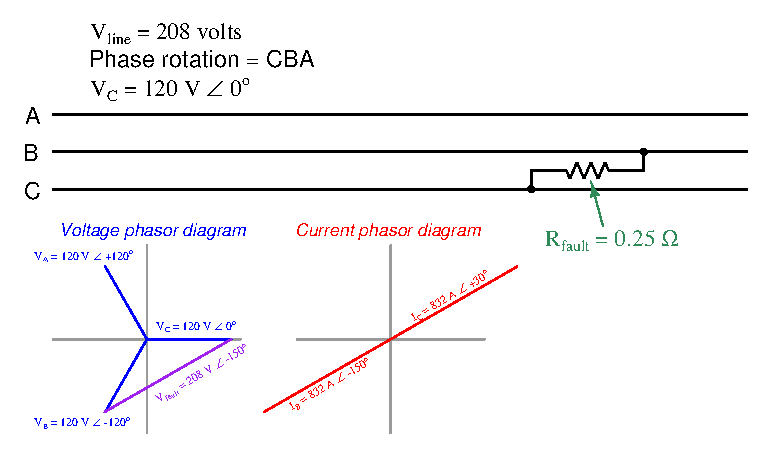
\includegraphics[width=15.5cm]{i00833x04.eps}$$

Det vises ingen fasor for leder A fordi uten tilkobling til denne linjen er $I_A = 0$.

%(END_ANSWER)





%(BEGIN_NOTES)


%INDEX% Electronics review: 3-phase electrical power 
%INDEX% Electronics review, phasor expressions of circuit quantities

%(END_NOTES)
